% settings.tex — Shared Beamer Config
%
% --- Base font size (edit to taste) ---
% Beamer accepts 8pt, 9pt, 10pt, 11pt (default), 12pt, 14pt, 17pt, 20pt.
% The value scales body text, frame titles, footnotes, and table fonts
% proportionally. Use a smaller value to fit more content per slide.
\documentclass[aspectratio=169,10pt]{beamer}

% Theme (use default unless overridden)
\usetheme{Madrid}
\usecolortheme{dolphin}

% Language and font
\usepackage[utf8]{inputenc}
\usepackage[T1]{fontenc}
\usepackage{lmodern}
% Math, figures, color, tables, and TikZ
\usepackage{amsmath, amssymb}
\usepackage{graphicx}
\usepackage{xcolor}
\usepackage{booktabs}
\usepackage{colortbl}
\usepackage{tikz}
\usepackage{float}

% Custom colors
\definecolor{myblue}{RGB}{0,70,140}
\setbeamercolor{structure}{fg=myblue}

% --- Slide margins (edit to taste) ---
% Beamer's defaults are ~1cm on each side; widen for a less cramped feel.
% Increase the values to push content further from the edges; decrease to fit
% wider tables/figures. Vertical breathing room is set by `frametitlemargin`.
\newlength{\slidemarginh}\setlength{\slidemarginh}{1.4cm}
\setbeamersize{text margin left=\slidemarginh, text margin right=\slidemarginh}
\setlength{\leftmargini}{1.5em}   % first-level itemize indent
\setlength{\leftmarginii}{1.3em}  % second-level itemize indent

% Footer customization (optional)
\setbeamertemplate{footline}[frame number]

% Note: enumitem is incompatible with beamer's enumerate machinery in
% recent versions (causes a \labelenumi recursion). We use beamer's
% built-in list spacing instead.

% Links
\usepackage{hyperref}
\hypersetup{colorlinks=true, urlcolor=myblue, linkcolor=myblue}


\usetikzlibrary{calc, arrows.meta}
\usepackage{float}
\usepackage{algorithm}
\newcommand{\G}{\mathcal{G}}
\title[Diagnosing Robustness of Decomposability in Gaussian Graphical Models]{Diagnosing Robustness of Decomposability \\ in Gaussian Graphical Models}
\author{Juan Carlos Cisneros \and Erik Sol\'e}
\institute{Universitat Pompeu Fabra}
\date{May 2026}

% Default to small body text — denser slides without crowding
\AtBeginDocument{\small}

% Compact list spacing
\setbeamertemplate{itemize/enumerate body begin}{\small}
\setbeamertemplate{itemize/enumerate subbody begin}{\footnotesize}

\begin{document}

% ========================================================================
\begin{frame}[plain]
    \titlepage
\end{frame}

% ========================================================================
\section{Introduction}

\begin{frame}{Motivation}
    \begin{itemize}
        \item Gaussian Graphical Models (GGMs) are the default tool to learn about conditional independence in graphical models.
        \item In class we explored frequentist inference. In this talk, we are concerned about Bayesian inference
        \item \textbf{Pros}: Uncertainty quantification
        \item \textbf{Cons}: Bayesian Inference over graphs is \textbf{hard} $\rightarrow$ Except when the graph is \textit{decomposable/chordal}
        \item \textbf{Trade-off:} Decomposability is a strong assumption. Most real graphs are not chordal, is this critical?
    \end{itemize}
\end{frame}

\begin{frame}{Overview}
    \begin{itemize}
        \item Go over Bayesian inference for Gaussian Graphical Models
        \item Assess performance of existing methods
        \begin{itemize}
            \item Empirical Bayes SAEM-MCMC of Donnet \& Marin (2012) for decomposable graphis
            \item BDGraph of Mohammadi \& Wit (2015) for general GGMs
        \end{itemize}
        \item Is chordality reasonable? What happens when it fails?
        \item Can we make use of the decomposable estimated graph?
        \item Propose a way to make use of the decomposable result as a diagnostic tool.
    \end{itemize}
\end{frame}

\begin{frame}{Decomposable Graphs}
    \tiny
    \begin{figure}[h]
    \centering
    % Define layers so we can draw colored blobs behind the nodes
    \pgfdeclarelayer{background}
    \pgfsetlayers{background,main}

    \begin{tikzpicture}[scale=1.6, auto, swap]
        % =========================================
        % LEFT: Non-Decomposable (The "Hole")
        % =========================================
        \begin{scope}[xshift=-2.5cm]
            % Nodes
            \node[draw, circle, fill=gray!20, thick] (1) at (0,2) {1};
            \node[draw, circle, fill=gray!20, thick] (2) at (2,2) {2};
            \node[draw, circle, fill=gray!20, thick] (3) at (2,0) {3};
            \node[draw, circle, fill=gray!20, thick] (4) at (0,0) {4};

            % Edges forming the 4-cycle
            \draw[thick, red] (1) -- (2) -- (3) -- (4) -- (1);

            % Label
            \node[align=center, below] at (1, -0.5) {\textbf{(a) Non-Decomposable Graph}\\ \footnotesize(A ``hole'': chordless 4-cycle)};

            % Visual cue for the hole
            \node[red, font=\huge] at (1,1) {$\times$};
        \end{scope}


        % =========================================
        % RIGHT: Decomposable with Cliques & Separators
        % =========================================
        \begin{scope}[xshift=2.5cm]
            % 1. Draw the Cliques in the background layer

            % 2. Draw Nodes on top (same positions as left)
            \node[draw, circle, fill=white, thick] (1b) at (0,2) {1};
            \node[draw, circle, fill=white, thick] (2b) at (2,2) {2};
            \node[draw, circle, fill=white, thick] (3b) at (2,0) {3};
            \node[draw, circle, fill=white, thick] (4b) at (0,0) {4};


                        \begin{pgfonlayer}{background}
                % Clique C1 = {1, 2, 3} (Top-Right Triangle) - Shaded Blue
                % Using a smooth plot to draw a blob around the nodes
                \filldraw[blue!30, opacity=0.5, draw=blue, dashed, line width=1pt]
                    plot [smooth cycle, tension=0.2] coordinates {
                        ($(1b)+(-0.2, 0.3)$)  % Above node 1
                        ($(2b)+(0.3, 0.3)$) % Top-right of node 2
                        ($(3b)+(0.3, -0.3)$) % Bottom-right of node 3
                    };

                % Clique C2 = {1, 3, 4} (Bottom-Left Triangle) - Shaded Red
                \filldraw[red!30, opacity=0.5, draw=red, dashed, line width=1pt]
                    plot [smooth cycle, tension=0.2] coordinates {
                        ($(1b)+(-0.2, 0.3)$) % Top-left of node 1
                        ($(3b)+(0.1, -0.2)$) % Bottom-left of node 3
                        ($(4b)+(0, -0.2)$)  % Below node 4
                    };
            \end{pgfonlayer}

            


            
            % 3. Draw Edges
            % Standard edges
            \draw[thick] (1b) -- (2b) -- (3b) -- (4b) -- (1b);
            % The Chord that makes it decomposable (highlighted)
            \draw[line width=2pt, purple!80!black] (1b) -- (3b);

            % 4. Add Labels for Cliques and Separator
            % Label C1 near node 2
            \node[blue!80!black, right] at ($(2b)+(0.4,0)$) {\normalsize $C_1=\{1,2,3\}$};

            % Label C2 near node 4
            \node[red!80!black, left] at ($(4b)+(-0.4,0)$) {\large $C_2=\{1,3,4\}$};

            % Label Separator pointing to the chord
            % The separator is the intersection: {1,3}
            \node[purple!80!black, align=center] (sepLabel) at (3, 1) {Separator\\$S_1 = C_1 \cap C_2$\\$S_1=\{1,3\}$};
            \draw[-{[length=3mm]}, purple!80!black, thick, bend right=20] (sepLabel.west) to ($(1b)!0.5!(3b)$);


            % Main Subfigure Label
            \node[align=center, below] at (1, -0.5) {\textbf{(b) Decomposable Graph}\\ \footnotesize(Decomposed into cliques)};
        \end{scope}

    \end{tikzpicture}
    \label{fig:decomposability_cliques}
\end{figure}

\end{frame}

% \begin{frame}{Bayesian Inference on graphs}
%     \begin{itemize}
%         \item At a high-level, nothing special about graphical models in a Bayesian setting.
%         \begin{itemize}
%             \item Specify likelihood $f(Y | \Sigma_G , G)$ and priors $\pi(\Sigma_G|G,\theta),\pi(G|\theta)$ for some parameters $\theta$.
%             \item Compute the posterior $\pi(G|Y) \propto \pi(G) \int f(Y|\Sigma_G , G) \pi(\Sigma_G|G)d\Sigma_G$
%         \end{itemize}
%         \item \textbf{Problem:} Under general conditions, conjugate priors need intractable normalizing constants $\rightarrow$ Inference becomes very computationally expensive.
%         \item \textbf{Workaround:} Decomposability $\implies$ that, for conjugate Hyper-Inverse-Wishart priors $\rightarrow$ Prior can be factorized over cliques and there are closed forms for the likelihood and the posteriors
%         \begin{itemize}
%             \item Drawing from the posterior becomes feasible and cheap
%         \end{itemize}
%     \end{itemize}
%     \begin{equation*}
%             \pi(G|Y,\delta,r,\Phi) \propto \frac{h_G (\delta,\Phi)}{h_G(\delta+n, \Phi + S_Y)}\pi(G|r)
%     \end{equation*}
%     \begin{itemize}
%         \item For estimation, we will do the following transformations $\delta = 1$ , $\Phi = \tau I_p$. Parameters to specify are thus $\tau$ and $r$. Can be understood as shrinkage and inclusion probability respectively.
%     \end{itemize}
% \end{frame}

\begin{frame}{Bayesian Inference on Gaussian Graphical Models}

\textbf{The setup:}
\begin{itemize}
    \item Likelihood: $Y \sim \mathcal{N}_p(0, \Sigma)$ with precision $\Omega = \Sigma^{-1}$
    \item Graph $G$ encodes zeros in $\Omega$: $\Omega_{ij}=0 \iff (i,j) \notin E$
    \item Prior on $(\Omega, G)$: G-Wishart $\times$ Bernoulli
\end{itemize}


\textbf{The goal:}
\[
\pi(G \mid Y) \propto \pi(G) \int p(Y \mid \Omega, G) \, p(\Omega \mid G) \, d\Omega
\]

\textbf{The problem:}
\begin{center}
\fbox{For general graphs, the integral over $\Omega$ has \textbf{no closed form}.}
\end{center}
\begin{itemize}
    \item The normalizing constant of the G-Wishart is intractable
    \item Inference requires costly approximations (MCMC within MCMC)
\end{itemize}

\textbf{The solution (for decomposable graphs):}
\begin{itemize}
    \item If $G$ is chordal, the G-Wishart \textbf{factorizes} over cliques and separators
    \item This yields a \textbf{closed-form} marginal likelihood (Hyper-Inverse Wishart)
    \item Posterior inference becomes exact and computationally feasible
\end{itemize}

\end{frame}
\begin{frame}{SAEM-MCMC procedure}
    \begin{itemize}
        \item Following Donnet and Marin (2012), we set $\delta=1$ and $\Phi = \tau I_p$.
        \item We have to set two parameters to specify the prior $r$ and $\tau$. These are prior inclusion probabilities for the edges and shrinkage respectively. We want to use Empirical Bayes (EB) so that their choice is data-driven. 
        \item We could take $    f(Y|\theta) \propto \sum_{G \in \mathcal{D}_p} \{\frac{h_G(\delta, \Phi)}{h_G(n+\delta, \Phi + S_Y)}\}\pi(G|r)$ and compute $\theta$. 
        \item However, we have to sum over the space of all decomposable graphs with $p$ vertices $\rightarrow$ Unfeasible for most $p$
        \item To overcome this, take a Stochastic Approximation Expectation Maximization (SAEM) approach
        \begin{itemize}
            \item By Gaussianity, this reduces to the approximation of three sufficient statistics
        \end{itemize}
        \item For SAEM, we need to simulate $(\Sigma_G^{(k)}, G^{(k)})$ from a suitable Markov Chain with target posterior $(\Sigma_G, G)|\hat\theta^{(k-1)}$ $\rightarrow$ Here we can use our specified priors and Metropolis Hastings.
        \item We iterate this procedure until convergence
    \end{itemize} 
\end{frame}

\begin{frame}{Sampling Graphs: Add and Delete}
    \begin{itemize}
        \item What do we mean by sampling $(\Sigma_G, G)$? For $\Sigma_G$ we use the HIW prior.
        \item To sample graphs, we use an \textit{add and delete} MH procedure:
        \begin{enumerate}
            \item Choose at random whether to delete or add and edge to the current graph
            \item If delete $\rightarrow$ Enumerate all possible \textbf{decomposable} graphs resulting from deleting an edge $\rightarrow$ Sample over that set with uniform probability
            \item If add $\rightarrow$ Enumerate all possible \textbf{decomposable} graphs resulting from adding an edge $\rightarrow$ Sample over that set with uniform probability
            \item Calculate the MH acceptance probability such that $\pi(G|Y,\theta)$ is the invariant distribution of the Markov Chain.
            \item With the corresponding acceptance probability, accept the draw of the new graph and continue iterating or keep the current graph.
        \end{enumerate}
        \item Note that we have a \textit{nested} iteration. For each approximated parameters we generate a graph and a covariance matrix. For each graph and covariance matrix we generate parameters by SAEM.
        \item Using the sufficient statistics and the graphical structure we can maximize the joint-likelihood using the updated values.
    \end{itemize}
\end{frame}


\begin{frame}{Misspecification and Robustness}
\begin{itemize}
    \item But what happens if the model is misspecified? What are we estimating?
    \item In practice, underlying structure is seldom decomposable.
    \item Is this critical? Is the estimated object uninterpretable?
    \item We leverage recent results of Niu et al (2020)
    \begin{itemize}
        \item Under suitable regularity conditions, the posterior becomes asymptotically supported on \textit{minimal triangulations} of the true $G$.
        \item Moreover, the "penalization" for missing a \textit{true} edge grows \textbf{exponentially} 
        \item The "penalization" for adding a \textit{false} edge grows \textbf{polynomially}
    \end{itemize}
    \item Under misspecification, we estimate a "wrong" graph, but the mistakes are structured $\rightarrow$ Wrong $\tilde G$ is a (weak) superset of the true $G$
    \item This gives us structure and intuition to explore the performance of the model.
    \item Moreover, it gives us some intuition about how to \textbf{use} the misspecified results in hopes of a better result.
\end{itemize}
\end{frame}

% ========================================================================

% ========================================================================
\section{The two-stage proposal}

\begin{frame}[t]{The two-stage proposal}
    \textbf{Stage 1.} Run SAEM-MCMC on $\mathcal{D}_p$. Returns the \textbf{Stage-1 PIP matrix} $\text{PIP}_{ij}$.
    \vspace{0.3cm}

    \textbf{Stage 2.} Run BDMCMC on the \emph{unrestricted} graph space, with the prior set by the \textbf{Decomposable-Informed Prior (DIP)}:
    \[
        \boxed{\;p_{ij} \;=\; \lambda\,\text{PIP}_{ij} \;+\; (1-\lambda)\, r_0\;}
    \]

    \begin{itemize}
        \item $(\lambda, r_0) = (0, 0.2)$ recovers the BDMCMC default (uniform Bernoulli prior)
        \item $\lambda > 0$ folds Stage-1 information into the Stage-2 prior
    \end{itemize}
    \vfill

    \textbf{The output:} two graphs from the same data:
    \[
        \hat G_D \in \mathcal{D}_p
        \quad \text{(decomposable)}
        \qquad \text{and} \qquad
        \hat G \in \mathcal{D}_p^{\,c} \cup \mathcal{D}_p
        \quad \text{(unrestricted)}
    \]
\end{frame}

% ========================================================================
\section{Evidence}

\begin{frame}[t]{Simulations}
    \footnotesize
    \begin{table}[H]
        \centering
        \begin{tabular}{lcccc}
            \toprule
            Topology & Stage-1 & BDMCMC & Two-stage (DIP) & GLASSO \\
            \midrule
            Chain (decomposable)               & 0.94 & \textbf{0.99} & 0.98 & 0.62 \\
            Star (decomposable)                & \textbf{0.98} & 0.96 & 0.95 & 0.18 \\
            Cycle (non-decomposable)           & 0.57 & \textbf{0.99} & 0.98 & 0.67 \\
            Erd\H{o}s--R\'enyi (non-decomp.)   & 0.77 & \textbf{0.97} & 0.95 & 0.59 \\
            Barab\'asi--Albert                 & 0.95 & \textbf{0.98} & 0.98 & 0.47 \\
            \bottomrule
        \end{tabular}
        \\[0.3em]
        \scriptsize
        Mean MCC over $p \in \{5, 10, 20\}$ and $5$ replicates, baseline calibration $d=5$ ($\rho_{\max} \approx 0.38$).
    \end{table}
    \vspace{0.2cm}

    \begin{itemize}
        \item Two-stage and BDMCMC differ by at most $0.03$ MCC at any topology
        \item The decomposability restriction (Stage-1 alone on cycle: $0.57$) is what hurts; lifting it via Stage 2 is what helps
        \item Robust across signal strength ($d \in \{3, 5, 10, 15\}$)
    \end{itemize}
\end{frame}

% ========================================================================
\begin{frame}[t]{Application: a misspecification verdict on the DDLY network}
    \textbf{Data.} Demirer, Diebold, Liu, and Yilmaz (2018) bank-volatility panel: $96$ banks and $10$ sovereign bonds, daily 2003--2014 ($n = 2{,}676$, $p = 106$).
    \vspace{0.2cm}

    Two-stage at $\lambda = 0.5$, $r_0 = 0.2$ (matching the simulation grid and $\lambda$-sensitivity sweep).
    \vspace{0.3cm}

    \footnotesize
    \begin{table}[H]
        \centering
        \begin{tabular}{lr}
            \toprule
            Quantity & Value \\
            \midrule
            Stage-1 edges (PIP $> 0.5$)                                      & $262$ \\
            Stage-2 edges (PIP $> 0.5$)                                      & $647$ \\
            Stage-1 graph decomposable?                                      & \textsc{true} \\
            Stage-2 graph decomposable?                                      & \textsc{false} \\
            Induced chordless 4-cycles in Stage-2                            & $3{,}742$ \\
            \rowcolor{yellow!30} Stage-2 added edges that break decomposability if added to $\hat G_D$ & $411\;(93.6\%)$ \\
            \bottomrule
        \end{tabular}
    \end{table}

    \begin{itemize}
        \item $94\%$ of the structure Stage-2 adds to Stage-1 explicitly violates decomposability
        \item The data demand a non-decomposable graph; the diagnostic detects it cleanly
        \item Qualitative claims should be read as descriptive, not asymptotically justified
    \end{itemize}
\end{frame}

% ========================================================================
\section{Takeaways}

\begin{frame}[t]{Takeaways}
    \vspace{0.2cm}
    \begin{enumerate}
        \item[\textbf{1.}] \textbf{The cost of decomposability is mild in moderate-$p$ settings.} The SAEM-MCMC posterior concentrates on the minimal triangulations of $G^*$, so meaningful structure is recovered. In higher dimensions decomposability becomes the binding restriction; on the DDLY panel at $p = 106$, the data prefer a non-decomposable graph.
        \vspace{0.25cm}
        \item[\textbf{2.}] \textbf{The two-stage output is itself a diagnostic.} Comparing the Stage-1 graph $\hat G_D$ against the unrestricted Stage-2 graph $\hat G$ flags misspecification of the decomposability assumption. On the DDLY panel, $94\%$ of Stage-2's added edges break Stage-1's decomposability. The diagnostic verdict is robust to the Stage-2 prior, even when the specific Stage-2 structure is not.
        \vspace{0.25cm}
        \item[\textbf{3.}] \textbf{A natural next step is a Bayesian test of decomposability.} Use the posterior mass on the decomposable subspace, $\mathbb{P}(G \in \mathcal{D}_p \mid Y)$ -- estimated as the fraction of post-burn-in Stage-2 samples that are decomposable -- as the test statistic, with the corresponding Bayes factor for $G \in \mathcal{D}_p$ vs.\ $G \notin \mathcal{D}_p$.
    \end{enumerate}
\end{frame}

% ========================================================================
\begin{frame}[plain]
    \begin{center}
        \vspace{1.5cm}
        {\Large Thank you}\\[0.6cm]

        \large Questions?
    \end{center}
\end{frame}

% ========================================================================
% Backup slides
% ========================================================================

\appendix

\begin{frame}[t]{Backup A: SAEM-MCMC algorithm}
    At iteration $k$:
    \begin{itemize}
        \item \textbf{S-step.} Generate $(G^{(k)}, \Sigma_G^{(k)})$ from MH transitions targeting $\pi(G, \Sigma_G \mid Y, \hat\theta^{(k-1)})$.
        \item \textbf{SA-step.} Update Robbins--Monro running averages of three sufficient statistics:
        \[
            S_1 = \sum_C |C|^2 - \sum_S |S|^2, \quad
            S_2 = \mathrm{tr}(\Sigma_G^{-1}), \quad
            S_3 = k_G
        \]
        \item \textbf{M-step.} Closed-form hyperparameter update:
        \[
            \hat\tau^{(k)} = \frac{(\delta - 1)p + s_1^{(k)}}{s_2^{(k)}},
            \qquad
            \hat r^{(k)} = \frac{s_3^{(k)}}{m}
        \]
    \end{itemize}
    \vfill
    \footnotesize
    Convergence (Kuhn \& Lavielle 2004): $\hat\theta \to$ a maximizer of $f(Y \mid \theta)$ a.s.\ provided the S-step invariant distribution is correct.
\end{frame}

% ========================================================================
\begin{frame}[t]{Backup B: $\lambda$-sensitivity sweep}
    \begin{center}
        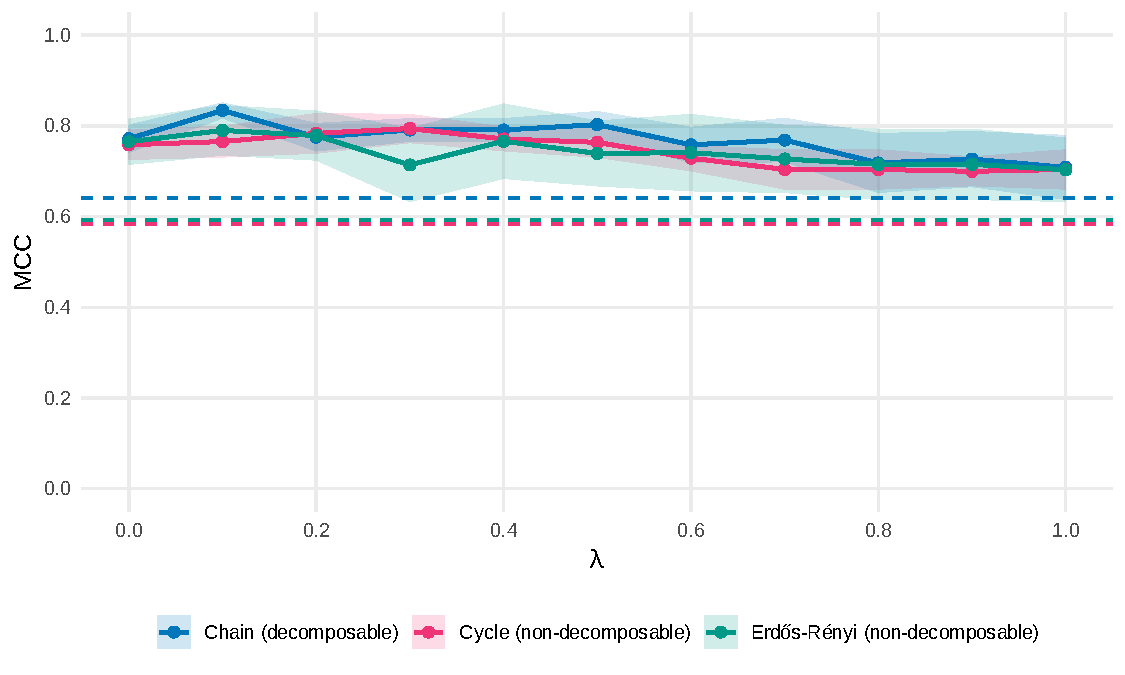
\includegraphics[width=0.78\textwidth, keepaspectratio, height=0.55\textheight]{../../2_analysis/output/figures/lambda_sensitivity.pdf}
    \end{center}
    \footnotesize
    Stage-2 MCC vs.\ DIP weight $\lambda$ at $p = 10$, $n = 500$, five replicates per topology. Dashed lines: Stage-1 baseline (independent of $\lambda$). $\lambda = 0$ is at or near the recovery optimum on every topology; gap to $\lambda = 1$ is $0.06$--$0.08$ MCC.
\end{frame}

% ========================================================================
\begin{frame}[t]{Backup C: top banks by Stage-2 degree centrality}
    \footnotesize
    \begin{table}[H]
        \centering
        \begin{tabular}{l r l}
            \toprule
            Bank & Degree & Region \\
            \midrule
            Regions Financial      & 23 & US (regional) \\
            Mizuho                 & 20 & Asia \\
            Royal Bank of Scotland & 19 & UK \\
            SunTrust               & 19 & US (regional) \\
            Deutsche Bank          & 18 & Eurozone \\
            Bank of America        & 18 & US (bulge) \\
            UBS                    & 18 & Other Europe \\
            Nordea                 & 17 & Other Europe \\
            KB Financial Group     & 17 & Asia \\
            Standard Bank Group    & 17 & Other EM \\
            \bottomrule
        \end{tabular}
    \end{table}
    \vfill
    Composition aligns with DDLY's ``to-degree'' systemic ranking. Their measure is dynamic and marginal, ours is contemporaneous and conditional, so the two estimands are related but not identical.
\end{frame}

\begin{frame}{Backup D: Sufficient Statistics and Likelihoods}
\begin{equation*}
    \pi((\Sigma_\G)_C | \delta, \Phi_C) = h_{\G_C}^{IW} [\det (\Sigma_\G)_C]^{-\frac{\delta+2|C|}{2}}\exp\{-\frac{1}{2}\text{tr}[(\Sigma_\G)_C^{-1} \Phi_C]\}
\end{equation*}
\begin{equation*}
    h_{\G_C}^{IW}(\delta, \Phi_C) = \frac{\det(\frac{\Phi_C}{2})^{(|C|+\delta-1)/2}}{\Gamma_{|C|}(\frac{|C| +\delta - 1}{2})}
\end{equation*}
\begin{equation*}
    h_G(\delta,\Phi) = \frac{\prod_{C\in \mathcal{C}}h_{G _C}^{IW} (\delta, \Phi_C)}{\prod_{S\in \mathcal{S}}h_{G_S}^{IW} (\delta, \Phi_S)}
\end{equation*}
\begin{equation}\label{margData}
    f(Y|\G, \delta,\Phi) = \frac{h_\G(\delta, \Phi)}{(2\pi)^{-np/2}h_\G (\delta+n, \Phi + S_Y)}
\end{equation}

    \begin{equation}
    \begin{gathered}
        S_1(Y, \G , \Sigma_\G) = \sum_{C\in\mathcal{C}} |C|^2 - \sum_{S\in\mathcal{S}}|S|^2\\
        S_2(Y, \G , \Sigma_\G) = \text{tr}(\Sigma_\G^{-1})\\
        S_3(Y, \G , \Sigma_\G) = k_\G
    \end{gathered}
\end{equation}
\end{frame}

\begin{frame}{Backup E: Add and Delete}
    \begin{algorithm}[H]
    \caption{Add and delete MH proposal}\label{alg:add-delete-mh}
    At iteration $t$
    \begin{enumerate}
        \item Choose at random (With equal probability) whether to delete or add an edge to $G^{(t-1)}$
        \begin{itemize}
            \item If an edge is deleted, enumerate $G_{G^{(t-1)}}^{-}$ and generate $G^p$ according to a uniform distribution on $G_{G^{(t-1)}}^{-}$
            \item If an edge is added, enumerate $G_{G^{(t-1)}}^{+}$ and generate $G^p$ according to a uniform distribution on $G_{G^{(t-1)}}^{+}$
        \end{itemize}
        \item Calculate the MH acceptance probability $\rho(G^{(t-1)}, G^p)$ such that $\pi(G| Y, \theta)$ is the invariant distribution of the Markov chain.
        \item With probability $\rho(G^{(t-1)}, G^p)$, accept $G^p$ and thus set $G^{(t)} = G^p$. Otherwise reject and set $G^{(t)} = G^{(t-1)}$
    \end{enumerate}
\end{algorithm}
\end{frame}

\begin{frame}{Backup F: Full MCMC algorithm}
    \begin{algorithm}[H]
    \caption{MCMC Algorithm}
    \begin{enumerate}
        \item Initialize $\hat\theta^{(0)}, s_1^{(0)}, s_2^{(0)},s_3^{(0)}$
        \item At each iteration $k$
        \begin{itemize}
            \item \ [S-Step]: Generate $\G^{(k)}$ and $\Sigma_\G^{(k)}$ from $M$ iterations of the MH procedure detailed in section 4.2
            \item \ [SA-Step]: Update $(s_i^{(k)})_{i=1,2,3}$ using the stochastic approximation scheme detailed in section 4.1
            \item \ [M-Step]: Maximize the joint-likelihood using the updated minimal sufficient statistics:
            \begin{equation*}
                \begin{gathered}
                    \hat\tau^{(k)} = \frac{(\delta-1)p + s_1^{(k)}}{s_2^{(k)}} \\
                    \hat r^{(k)} = \frac{s_3^{(k)}}{m}
                \end{gathered}
            \end{equation*}
        \end{itemize}
        \item Set $k = k+1$ and repeat until convergence
    \end{enumerate}
\end{algorithm}

\end{frame}

\end{document}
